\documentclass[twocolumn]{article}
\setlength{\columnsep}{40px}

\usepackage{graphicx}
\usepackage{listings}
\usepackage{listings-rust}
\usepackage{color}

\definecolor{dkgreen}{rgb}{0,0.6,0}
\definecolor{gray}{rgb}{0.5,0.5,0.5}
\definecolor{mauve}{rgb}{0.58,0,0.82}

\lstset{frame=tb,
  language=Rust,
  aboveskip=3mm,
  belowskip=3mm,
  showstringspaces=false,
  columns=flexible,
  basicstyle={\small\ttfamily},
  numbers=none,
  numberstyle=\tiny\color{gray},
  keywordstyle=\color{blue},
  commentstyle=\color{dkgreen},
  stringstyle=\color{mauve},
  breaklines=true,
  breakatwhitespace=true,
  tabsize=3
}


\graphicspath{ {./} }

\title{XycLoans: Flash Loans and \\ Liquidity Protocol on Soroban}
\author{
    The Xycloo Labs team.
    \vspace{1.5cm}
}
\date{}

\begin{document}

\maketitle


\abstract{XycLoans is a decentralized network that brings flash loans to Soroban. The protocol achieves liquidity efficiency for multiple tokens through its vaults and liquidity provider rewards.
}


\vspace{30px}

\section{Introduction}
Decentralized Finance, or DeFi, benefits from large amounts of capital: arbitraging for price leveling across protocol swaps, collateral debt position liquidation to protect lenders, efficient operations to limit fees for end users, and trading tactics in general also benefit from large amounts of capital, like efficient collateral swapping or CDP unwinding.

\

All these actions don't require the capital to be permanently held by the executing operation's source, but can also be borrowed. However, debt positions in decentralized finance need to be backed by collateral as there is no other guarantee on the borrower's end. 

Operations like successful arbitrage are thus only possible for investors with significant assets, limiting the market efficiency.

\

Flash loans allow for uncollateralized borrows without exposing lenders to the risk of losing their capital.

\vspace{20px}

\section{How Flash Loans Work}
Uncollateralized borrowing is possible thanks to a smart contract's ability to revert a state-changing transaction in the event that a particular condition is or is not met. This allows a contract to lend money and revert the transaction if the borrower doesn't return the money plus interest.

\

Flash loans thus happen within one transaction, which will fail if the borrower can't repay the loan. Later sections of the document will discuss how flash loans can be used in decentralized finance.

\vspace{20px}

\section{Protocol Overview}
The protocol is accessed through a proxy that makes discoverability more structured and allows for efficient contract upgradeability. The proxy stores a flash loan contract id and a vault contract id for each token that can be borrowed through the protocol. The proxy contract is controlled by the protocol contract that, controlled by governance, can edit the proxy's values, so upgrading contracts. 

Every action that takes place in the protocol on the borrower's and lender's side happens by invoking the proxy contract.

The graphic below describes how the protocol is organized.

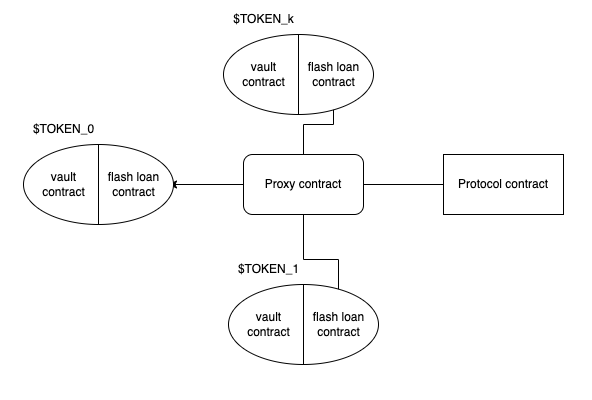
\includegraphics[scale=0.35]{protocol}

\vspace{20px}

\section{Borrowing: Flash Loans}

The borrowing trait of the protocol resides in its flash loans. Users invoke the proxy contract specifying the token to borrow, the amount, and the receiver contract. The proxy will then map the token to a flash loan contract and invoke it, resulting in the flash loan transferring the specified amount to the receiver contract. 

Subsequently, the flash loan will invoke the receiver contract, which will perform a predefined set of operations using the borrowed capital. At the end of its execution, the receiver sets up an allowance with the flash loan contract as spender and as amount the borrowed amount \(+\) fixed governance-agreed interest.

\subsection{The Receiver Contract}

The receiver contract has to expose a \texttt{exec\_op} method that performs the wanted operations. We also provide a receiver interface trait to be optionally imported and implemented in receiver contracts.

\begin{lstlisting}
// flash loan receiver interface

use crate::types::ReceiverError;
use soroban_sdk::{contractimpl, Env};

#[doc = "Standard interface for FlashLoan receivers. Implementing `exec_op` is mandatory, but you can also extend the contract for better developer experience, for example, having an `init` function to store all the values instead of hard-coding them could be a good idea."]
pub trait FlashLoanReceiverTrait {
    #[doc = "The method invoked by the FlashLoanLender contract. Here @dev should implement the logic behind how the borrowed amount is going to be used."]
    fn exec_op(env: Env) -> Result<(), ReceiverError>;
}

pub struct FlashLoanReceiver;

#[contractimpl]
impl FlashLoanReceiverTrait for FlashLoanReceiver {
    fn exec_op(env: Env) -> Result<(), ReceiverError> {
        Ok(())
    }
}
\end{lstlisting}

\vspace{20px}

\section{Lending: Liquidity Management and Cash Flow}

Liquidity management is a key factor in the protocol, and is managed by vaults. A vault is a contract that receives the interest that the respective token's flash loan earns. The interest is referred to as fees, and the vault takes care of withdrawing them to the flash loan's liquidity providers.

The vault has three functionalities:
\begin{itemize}
\item depositing liquidity
\item withdrawing yield
\item withdrawing the whole liquidity position.
\end{itemize} 

\subsection{Depositing}
When a provider makes a deposit, the deposited amount will go to the flash loan's balance and the vault will mint fee shares to the provider according to (1).

\begin{equation}
minted = \frac{a \cdot S}{B}
\end{equation}

Where
\begin{itemize}
\item \(a\) is the deposited amount.
\item \(S\) is the total circulating supply of the fee shares
\item \(B\) is the current balance of the vault \( + \) the balance of the flash loan contract.
\end{itemize}

Fee shares are minted inside batches that are stored in the vault's storage. These batches keep track of the number of fee shares that are circulating within that batch, the amount of shares initially minted for the batch, and the amount that was deposited to mint the shares. 

Every time that a provider withdraws their fee shares, they will be minted new ones in another batch. These newly minted fee shares refer to the portion of liquidity that generated the withdrawn yield. 

As a result, a provider could also withdraw only a portion of a batch's fees, get new shares minted and have two active fee batches that will hold different values.

\subsection{Withdrawing Yield}

As mentioned, liquidity providers use fee shares to withdraw yield: the vault sends an amount of the fee pool to the liquidity providers when they burn fee shares.

The amount \( fee(x) \) of the fee pool sent to the collector is calculated with (2).

\begin{equation}
fee(n) = \frac{B \cdot x }{S} - D \cdot \frac{x}{i}
\end{equation}

Where
\begin{itemize}
\item \( n \) is the number of fee shares being burned
\item \( i \) is the number of fee shares that were initially minted in the batch
\item \( S \) is the total circulating supply of the fee shares
\item \( B \) is the current balance of the vault \( + \) the balance of the flash loan contract.
\end{itemize}

When the liquidity provider has their fees among multiple batches, and want to withdraw them all, the vault offers a function that calculates the total amount of fees \( F \) their are entitled to. The calculation is done by (3)

\begin{equation}
F = \sum_{k}^{batches} fee (c_k)
\end{equation}

Where
\begin{itemize}
\item \( c_k \) is the circulating supply of the shares in the batch \( k \)
\end{itemize}

\subsubsection{Re-Minting the fee shares}
Once the liquidity provider has burned \( n \) fee shares, they should still be entitled to a portion of the future interest accumulated in the flash loan. That's because the principal (or initial deposit) referring to the burned shares remains in the flash loan and keeps generating new yield. 

\

This is accomplished by minting a new batch \(k\), where its deposit is calculated with (4) and its initial shares are calculated with (5).

\begin{equation}
D_{k} = D \cdot \frac{n}{i}
\end{equation}

Where
\begin{itemize}
\item \( D \) is the deposit of the batch that burned the shares
\item \( n \) is the amount of shares that were burned
\item \( i \) is the initial amount of shares of the batch that burned the shares
\end{itemize}

\begin{equation}
minted_{k} = \frac{D_{k} \cdot S}{B - D_{k}}
\end{equation}

Where
\begin{itemize}
\item \( D_{k} \) is the above calculated deposit for the new batch
\item \( S \) is the current total circulating supply of the fee shares
\item \( B \) is the current balance of the vault \( + \) the balance of the flash loan contract.
\end{itemize}

\subsection{Withdrawing Liquidity Position}
When the liquidity provider wishes to stop providing liquidity for the protocol, the vault offers a function to collect all their fees (that might be sparse within different batches) and return their principal as well.

The amount that the liquidity provider receives from the protocol after calling this function is calculated with (5).

\begin{equation}
Amount = D_{initial} + F
\end{equation}

Where
\begin{itemize}
\item \( D_{initial} \) is the liquidity the liquidity provider initially sent to the flash loan, or principal
\item \( F \) is the total amount of the liquidity provider's fees across batches, calculated with (3)
\end{itemize}

\vspace{20px}

\section{Building with Flash Loans in DeFi}
Flash loans are still a relatively new technology and developers are pioneering new use cases, but there already are well-known techniques that traders and developers use everyday to profit from market opportunities or save gas.

In the next subsections we briefly discuss some of these use cases as proof of what the ecosystem can build with XycLoans.

\subsection{Arbitrage Trading}

These opportunities occur if there are price differences from one marketplace to another. Traders can then take advantage of that by buying at a lower price and selling at a higher one. In an efficient ecosystem it is almost always only profitable if executed with large amounts of capital.

Flash loans allow to perform arbitrage trading without needing large amounts of capital, which is healthy for the overall market since it helps leveling the price between various marketplaces.

\subsection{Collateralized Debt Position Liquidation}
The Lending/Borrowing ecosystem in decentralized finance is based on collateral. Borrowers lock in collateral and borrow a certain amount of a token, usually around the value of the 80\% of the locked collateral.

Borrowing power increases when the deposited collateral's price does, and diminishes when the deposited collateral decreases in price. To incentivize lenders and for overall protocol wealth, protocols use liquidations: when a debt position decreases by a certain value, a liquidation can happen, meaning that any user can pay back another user's debt and receive the collateral and a liquidation fee as well.

With flash loans, one can easily liquidate debt positions and trade the collateral(s) for the best price without needing a large amount of capital.

This obviously opens up the window for self-liquidation, so a user could close their collateralized debt position  with a flash loan rather than letting it enter liquidation phase.

\subsection{Efficient Collateral Swapping}
Money markets tend to allow swapping your collateral for trading purposes. Unless you already have the capital to make the swap happen, this would mean having to pay back your debt, swap your collateral, and open a new debt position with the new token, which is unfortunate and will cost you more fees.

Fortunately, with flash loans you could borrow money to swap the collateral and receive your previously-locked tokens. Then re-pay the flash loan lender + a small fee.


\subsection{Unwinding a Debt Position}
With flash loans borrowers can unwinding a collateralized debt position by borrowing from the flash loan, paying back part of the debt, unlock some of the collateral, trade it for the best price and finally re-pay the flash loan.

Flash loans are handy here since they allow to perform this operation without having additional capital to pay part of the debt position.

\end{document}
